% !TEX TS-program = pdflatex
% !TEX root = ../tesi.tex

%************************************************
\chapter{Introduzione}
%\label{chp:Introduzione}
%************************************************

%This chapter introduces the (truly simple) basic notions of \arsclassica{} and presents its fundamental ideas and distinctive features.
L’inquinamento acustico marino è causato dall’immissione di rumori in quantità eccessiva rispetto a quanto l’ambiente in questione sia in grado di sopportare. Vari studi dimostrano che i rumori provocati dall’uomo siano quelli che provocano più effetti negativi sui vari organismi marini. In particolare, le principali fonti di inquinamento marino sono rappresentate dall’attività di ricerca di combustibili fossili (come gas e petrolio), dai sonar utilizzati per usi militari o civili, dalla costruzione di edifici sulla costa, dall’attività di pesca, dagli impianti eolici e infine dal traffico marittimo (che è in costante aumento, in particolare nel Mar Mediterraneo).
Gli impatti di tutte queste attività possono essere diversi a seconda del tipo di rumore prodotto, di dove esso è localizzato e della sua durata. I rumori provocati dai sonar, ad esempio, possono causare dei danni diretti (come una sordità temporanea o permanente). Tuttavia, anche i rumori più deboli non sono da sottovalutare perché, seppur in modo non immediato e meno evidente, anch’essi possono avere effetti negativi importanti, soprattutto se la loro durata è lunga e/o continua. Inoltre, data l’importanza del suono per gli animali marini e la capacità di propagazione del suono nel loro habitat, l’inquinamento acustico nel mare può avere conseguenze non solo sul singolo individuo, ma sull’intera popolazione marina.
%\section{Introduzione}
%The \arsclassica{} package changes some features of the \classicthesis{} style, designed by Andr\'e Miede. It allows to reproduce the layout of the \LaTeX{} guide \emph{The Art of Writing with \LaTeX}~\parencite{pantieri:arte} and of this document.
\chapter{Cenni Storici}
\subsection{L'idrofono}
Un idrofono è uno strumento elettroacustico per rivelare suoni in un liquido (generalmente acqua) e determinare la direzione della loro sorgente. il principio di funzionamento è simile a quello del microfono che in aria trasforma le vibrazioni di una sottile membrana dovute al transito dell’onda acustica, in segnali elettrici elaborabili. In acqua la membrana è sostituita da un diverso trasduttore. Negli idrofoni comuni si utilizzano sensori piezoelettrici nei quali la pressione dell’onda acustica sulle superfici di un opportuno materiale cristallino genera un segnale elettrico.

Questo strumento è largamente utilizzato in marineria per rivelare la presenza di navi tramite la ricezione dei rumori subacquei generati dall'elica in movimento e dai motori. Gli idrofoni furono sviluppati in modo intensivo durante la guerra 1914-18 per consentire ai cacciasommergibili di scoprire la presenza di sommergibili nemici immersi. Lo sviluppo dell’idrofono avvenne contemporaneamente in vari paesi, dunque non ne esiste un unico, definito inventore. 
Vanno ricordati: L. Nixon che per primo cercò di rivelare la presenza di iceberg con un rivelatore passivo di suoni (1906), A Blem in Vienna (1912), Lewis Richardson in Gran Bretagna (1913 primo brevetto eco-scandaglio) , il canadese Reginald Fessenden negli Stati Uniti (1914 primo SONAR), Il fisico francese Paul Langévin e Constantin Chilowsky ingegnere russo immigrato in Francia (brevetto di un SONAR che battezzarono hydrophone 1915) e, infine, il fisico canadese R.W. Boyle , studioso di ultrasuoni e delle loro applicazioni alla University of Alberta, che dal 1916 brevettò un SONAR poi ulteriormente sviluppato dallo stesso R.W. Boyle nei laboratori della Royal Navy. Nel 1918 il gruppo di Boyle sviluppò un SONAR capace di individuare la presenza di sommergibili ad una distanza di 1800 metri che venne installato negli anni successivi sulle unità della marina inglese.

Questo strumento si è diffuso moltissimo, non solo per i possibili usi militari, ma anche negli studi oceanografici, nelle ricerche biologia marina, nella protezione dei parchi marini, nella prevenzione dai terremoti e dagli tsunami, e in tutta la marineria commerciale e turistica. L’idrofono è infatti l’unità ricevente di ogni eco-scandaglio, uno strumento di grande uso, presente ormai in ogni imbarcazione di diporto per identificare gli scogli sommersi, la presenza di branchi di pesci o la profondità della scogliera.

Nell’acque marine in superficie e ad una temperatura di 20 °C il suono si trasmette ad una velocità di circa 1521 metri al secondo cioè 4,5 volte superiore a quella nell'aria. L’assorbimento del suono in acqua è invece molto minore. Oggi gli idrofoni, anche grazie allo sviluppo delle moderne tecniche di trasformazione dell’onda sonora in segnale elettronico o opto-elettronico, consentono quindi di captare anche suoni emessi a grandi distanze. La direzione della sorgente viene determinata dallo sfasamento dell’onda sonora tra idrofoni posti a vari metri di distanza.

Più complesso è determinare la distanza della sorgente. Il metodo utilizzato è quello di misurare il tempo che impiega un’onda sonora a raggiungere il corpo da monitorare e a ritornare riflessa alla sorgente. In questo caso si può scoprire la presenza e determinare la distanza di un oggetto in acqua anche se esso non produce onde sonore: è quanto avviene negli eco-scandagli o nei sonar. L’idrofono è l’unità ricevente anche di molti altri strumenti usati in ingegneria idraulica come, ad esempio, misuratori di portata, di pressione in condutture idrauliche o di sensori per la rilevazione di correnti in profondità in bacini marini o lacustri.

Gli idrofoni sono largamente diffusi nelle ricerche di biologia marina per conoscere abitudini e tracciare le migrazioni dei grandi cetacei, delle balene o dei delfini senza introdurre perturbazioni o presenze inadatte al loro habitat naturale, o anche per studiare l’utilizzo della comunicazione sonora dei mammiferi marini. Sono anche utilizzati per misurare temperatura, salinità e pressione (direttamente correlata 
con la profondità) locali. La velocità dell’onda acustica varia infatti con le proprietà dell’acqua. 
Ad esempio: un aumento di 1°C grado Celsius  dell’acqua marina determina un aumento della velocità dell’onda acustica di 4 metri al secondo, la variazione di pressione dovuta a un chilometro di inabissamento provoca una crescita della velocità di 1,4 metri al secondo. Le variazioni globali del clima sono controllabili tramite la tomografia acustica di vaste zone degli oceani (milioni di chilometri quadrati). Idrofoni sono anche utilizzati per la protezione da terremoti terrestri. 
L’idrofono ha una sua ampia utilizzazione nei modem acustici per la trasmissioni dati attraverso l’acqua. Le onde radio non si trasmettono sottacqua, i sistemi di trasmissione dati sommersi sono quindi basati sulla trasmissione cablata (fibre ottiche) o su quella sonora. Nei modem acustici si tratta di trasformare un segnale digitale in onde sonore, e poi di riconvertirlo. Come accade con la tradizionale “modulazione” sulle linee telefoniche analogiche (quella che usa uno strumento chiamato modem, cioè un modulatore e de-modulatore). I modem acustici, quantunque la velocità di trasmissione sia molto inferiore a quella dell’onda elettromagnetica in aria (onde radio) o su cavo, realizzano attualmente una ottima soluzione alla trasmissione dati wireless in acqua tra stazioni sommerse (subsea) e dall’acqua da stazioni sommerse ad una centrale emersa (topsea). Questi nuovi sistemi sono di grande utilità nell’oceanografia e in molte altre applicazioni scientifiche, civili e militari e sono quindi in grande, rapida, espansione. 

Idrofoni di particolare sensibilità sia con le tradizionali tecniche pizio-elettriche , sia con innovative tecniche FBG utilizzano fibre ottiche con reticoli di Bragg (FBG) , sono oggi proposti per essere utilizzati in ricerche di fisica sub-nucleare o astrofisica per rilevare il passaggio di particelle in un mezzo liquido.
\begin{code}
\end{code}
\subsection {Sonar e la sua nascita}
Venne inventato da Paul Langevin nel 1917. La marina inglese e quella tedesca considerarono il sottomarino, nel periodo tra le due guerre, un'arma superata soprattutto dopo l'avvento del dispositivo di rilevazione acustica detto "ASDIC" (Anti-Submarine Detection Investigation Committee), noto oggi come sonar; furono i britannici i primi a sviluppare una tecnologia che permettesse di rilevare un oggetto attraverso il suono, e la scoperta del propagarsi delle onde sonore in acqua non era avvenuta durante la prima guerra mondiale e, per il rilevamento dei sommergibili, erano utilizzati dei semplici idrofoni). Il sistema ASDIC era composto da un trasduttore, contenuto in una cupola sotto la nave, che inviava onde acustiche che tornavano all'origine se riflesse da un oggetto sommerso, posto ad una distanza massima di circa 
2700 m. La cupola poteva essere fissa, come nell'apparato Type 123 installato sulle corvette della classe Flower o retrattile come in alcune navi, quali il cacciatorpediniere HMS Campbeltown, dotato di un ASDIC Type 124. Dall'eco veniva ricavata la direzione e la distanza dell'oggetto ma falsi segnali potevano essere generati dalle differenze di temperatura dell'acqua, correnti, banchi di pesci (strato riflettente profondo), ed inoltre l'ASDIC era efficace solo a velocità inferiori ai 15 nodi (28 km/h), poiché a velocità superiori il rumore della nave avrebbe coperto gli echi; un ulteriore limite era rappresentato dal brandeggio del trasduttore, solo in senso orizzontale, con la conseguenza che il contatto veniva perso quando il bersaglio passava sotto la nave cacciatrice.

La procedura di utilizzo consisteva nell'uso dell'ASDIC in un arco da un lato all'altro della nave, fermando il trasduttore a distanze di pochi gradi per inviare un segnale, e le ricerche in gruppi di navi prevedevano l'allineamento delle navi a distanza compresa tra il miglio ed il miglio e mezzo; se veniva captata un'eco identificabile come sottomarino la nave avrebbe puntato verso il bersaglio e si sarebbe avvicinata a media velocità fino a trovarsi ad una distanza inferiore alle 1000 yard (910 m) e, nel frattempo, tramite il plotter veniva tracciata la direzione e la distanza, in modo da ricavare la rotta del sottomarino e la sua velocità. L'attacco veniva portato passando davanti al sottomarino per scaricare le bombe di profondità, lanciandole ad intervalli, seguendo uno schema tale da intrappolare il sottomarino. Per essere efficaci tuttavia, le bombe dovevano esplodere ad una distanza inferiore ai 6 metri e i primi sistemi ASDIC non erano in grado di determinare la profondità con sufficiente precisione; per questo motivo lo schema di sganciamento delle bombe prevedeva anche l'esplosione delle stesse a diverse profondità.

Il sistema ASDIC soffriva di alcuni limiti: 
gli U-Boot potevano scendere a profondità maggiori rispetto a quelli britannici e statunitensi, pari a 210 m, oltre le capacità delle bombe di profondità britanniche, che potevano raggiungere circa 100 m, e l'esplosione di una bomba di profondità disturbava l'acqua, rendendo molto difficile la riacquisizione del contatto nemico se falliva il primo attacco; è da rilevare inoltre che il sistema non godeva della fiducia delle marine alleate e la Royal Navy iniziò la guerra con un numero insufficiente di cacciatorpediniere e di ufficiali esperti in armi antisommergibile. La situazione nel comando costiero della Royal Air Force era ancora più grave, poiché gli aerei da ricognizione non possedevano adeguata autonomia per il pattugliamento e non erano ancora state valutate le conseguenze che la scoperta del radar avrebbe avuto nella guerra sul mare.

Anche altre marine iniziarono a sperimentare i primi modelli di ASDIC quando alcune unità, corvette ma anche pescherecci armati, vennero equipaggiati con personale non inglese, o apparati vennero installati su navi alleate, come il cacciatorpediniere olandese Isaac Sweers.

In Italia lo studio e la costruzione dei sonar riprende dopo la seconda guerra mondiale nel 1951.

I primi sonar italiani per sottomarini, costruiti tra il 1960 e 1974, erano identificati con le sigle: IP60 - IP64 e IP70 - IP74S. Il loro nome, coniato in Italia, era: Apparati Ecoidrofonici.
\begin{figure}
\centering 
\subfloat [Sottomarino CI. Toti (1967)]
{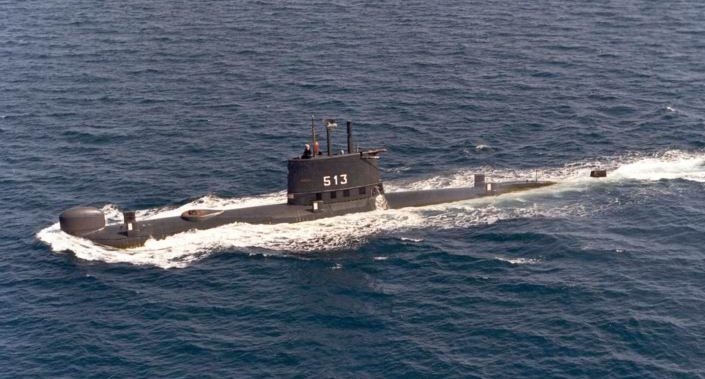
\includegraphics[width=.45\columnwidth]{SOTTOMARINO CI 1967}} \quad
\subfloat [Sottomarino CI Sauro (1976)]
{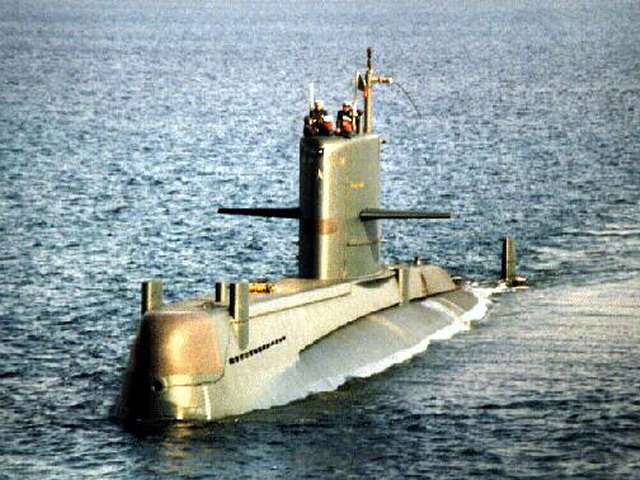
\includegraphics[width=.45\columnwidth]{SOTTOMARINO CI SAURO}} \quad
\subfloat[Sottomarino CI U212 (2003)]
{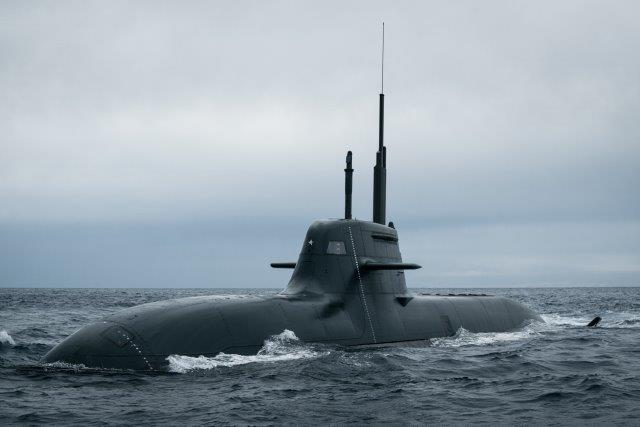
\includegraphics[width=.45\columnwidth]{SOTTOMARINO CI}} \quad
\caption [Sottomarini in italia dal 1960 ad oggi]{Sottomarini in Italia dal 1960 ad oggi}
\end{figure}

\chapter{Applicazione}
\subsection{Obiettivi}
Gli obiettivi di questa ricerca, con l’utilizzo dell’idrofono, sono quelli di evidenziare come il rumore ripreso sul fondo del mare, possa riscontrare problematiche a livello acustico di un certo tipo.
Gli idrofoni vengono utilizzati per misurare il rumore antropogenico, come quello prodotto dalle navi, e il suo impatto sull'ambiente marino, qui in Puglia, è davvero notevole;
La ricerca è la parte fondamentale di questo studio, infatti inizialmente la ricerca si è improntata sulla costruzione di un idrofono, con l'utilizzo di piezoelettrici bilanciati, collegati ad un XRL, con l'utilizzo di una scheda audio e di un computer, per effettuare delle registrazioni. 
In merito ai risultati ottenuti, si sono svolte poi altre ricerche e conclusioni, che hanno portato a conclusioni importanti: 

\begin{itemize}
\item La costruzione di un idrofono più professionale con l'utilizzo di piezoelettrici cilindrici in ceramica\ 
\item l'acquisto di un idrofono professionale tramite aziende specializzate nel settore
\item Ricerca di informazioni e dati dai Centri Nazionali di Ricerca nell'ambito della bioacustica e sopratutto specializzati nel rumore. 
\end{itemize}

Dopo svariate ricerche e consulenze in merito, la giusta scelta e sopratutto quella che avrebbe aiutato nello scopo è stata quella di fare ricerchè in merito a Centri Nazionali di Ricerca, Università, e associazioni specializzate nello studio dell'acqua e sopratutto nel mondo del monitoraggio ambientale marino. 

\subsection{Ricerca e studi}
Inizialmente la ricerca è stata effettuata su che suono avesse l'acqua. Da questo, il protagonista principale è stato l'idrofono. 
Insieme al mio relatore l'applicazione iniziale è stata quella di costruirne uno per effettuare delle registrazioni;

\begin{figure}
\centering
\subfloat[Idrofono fai da te]
{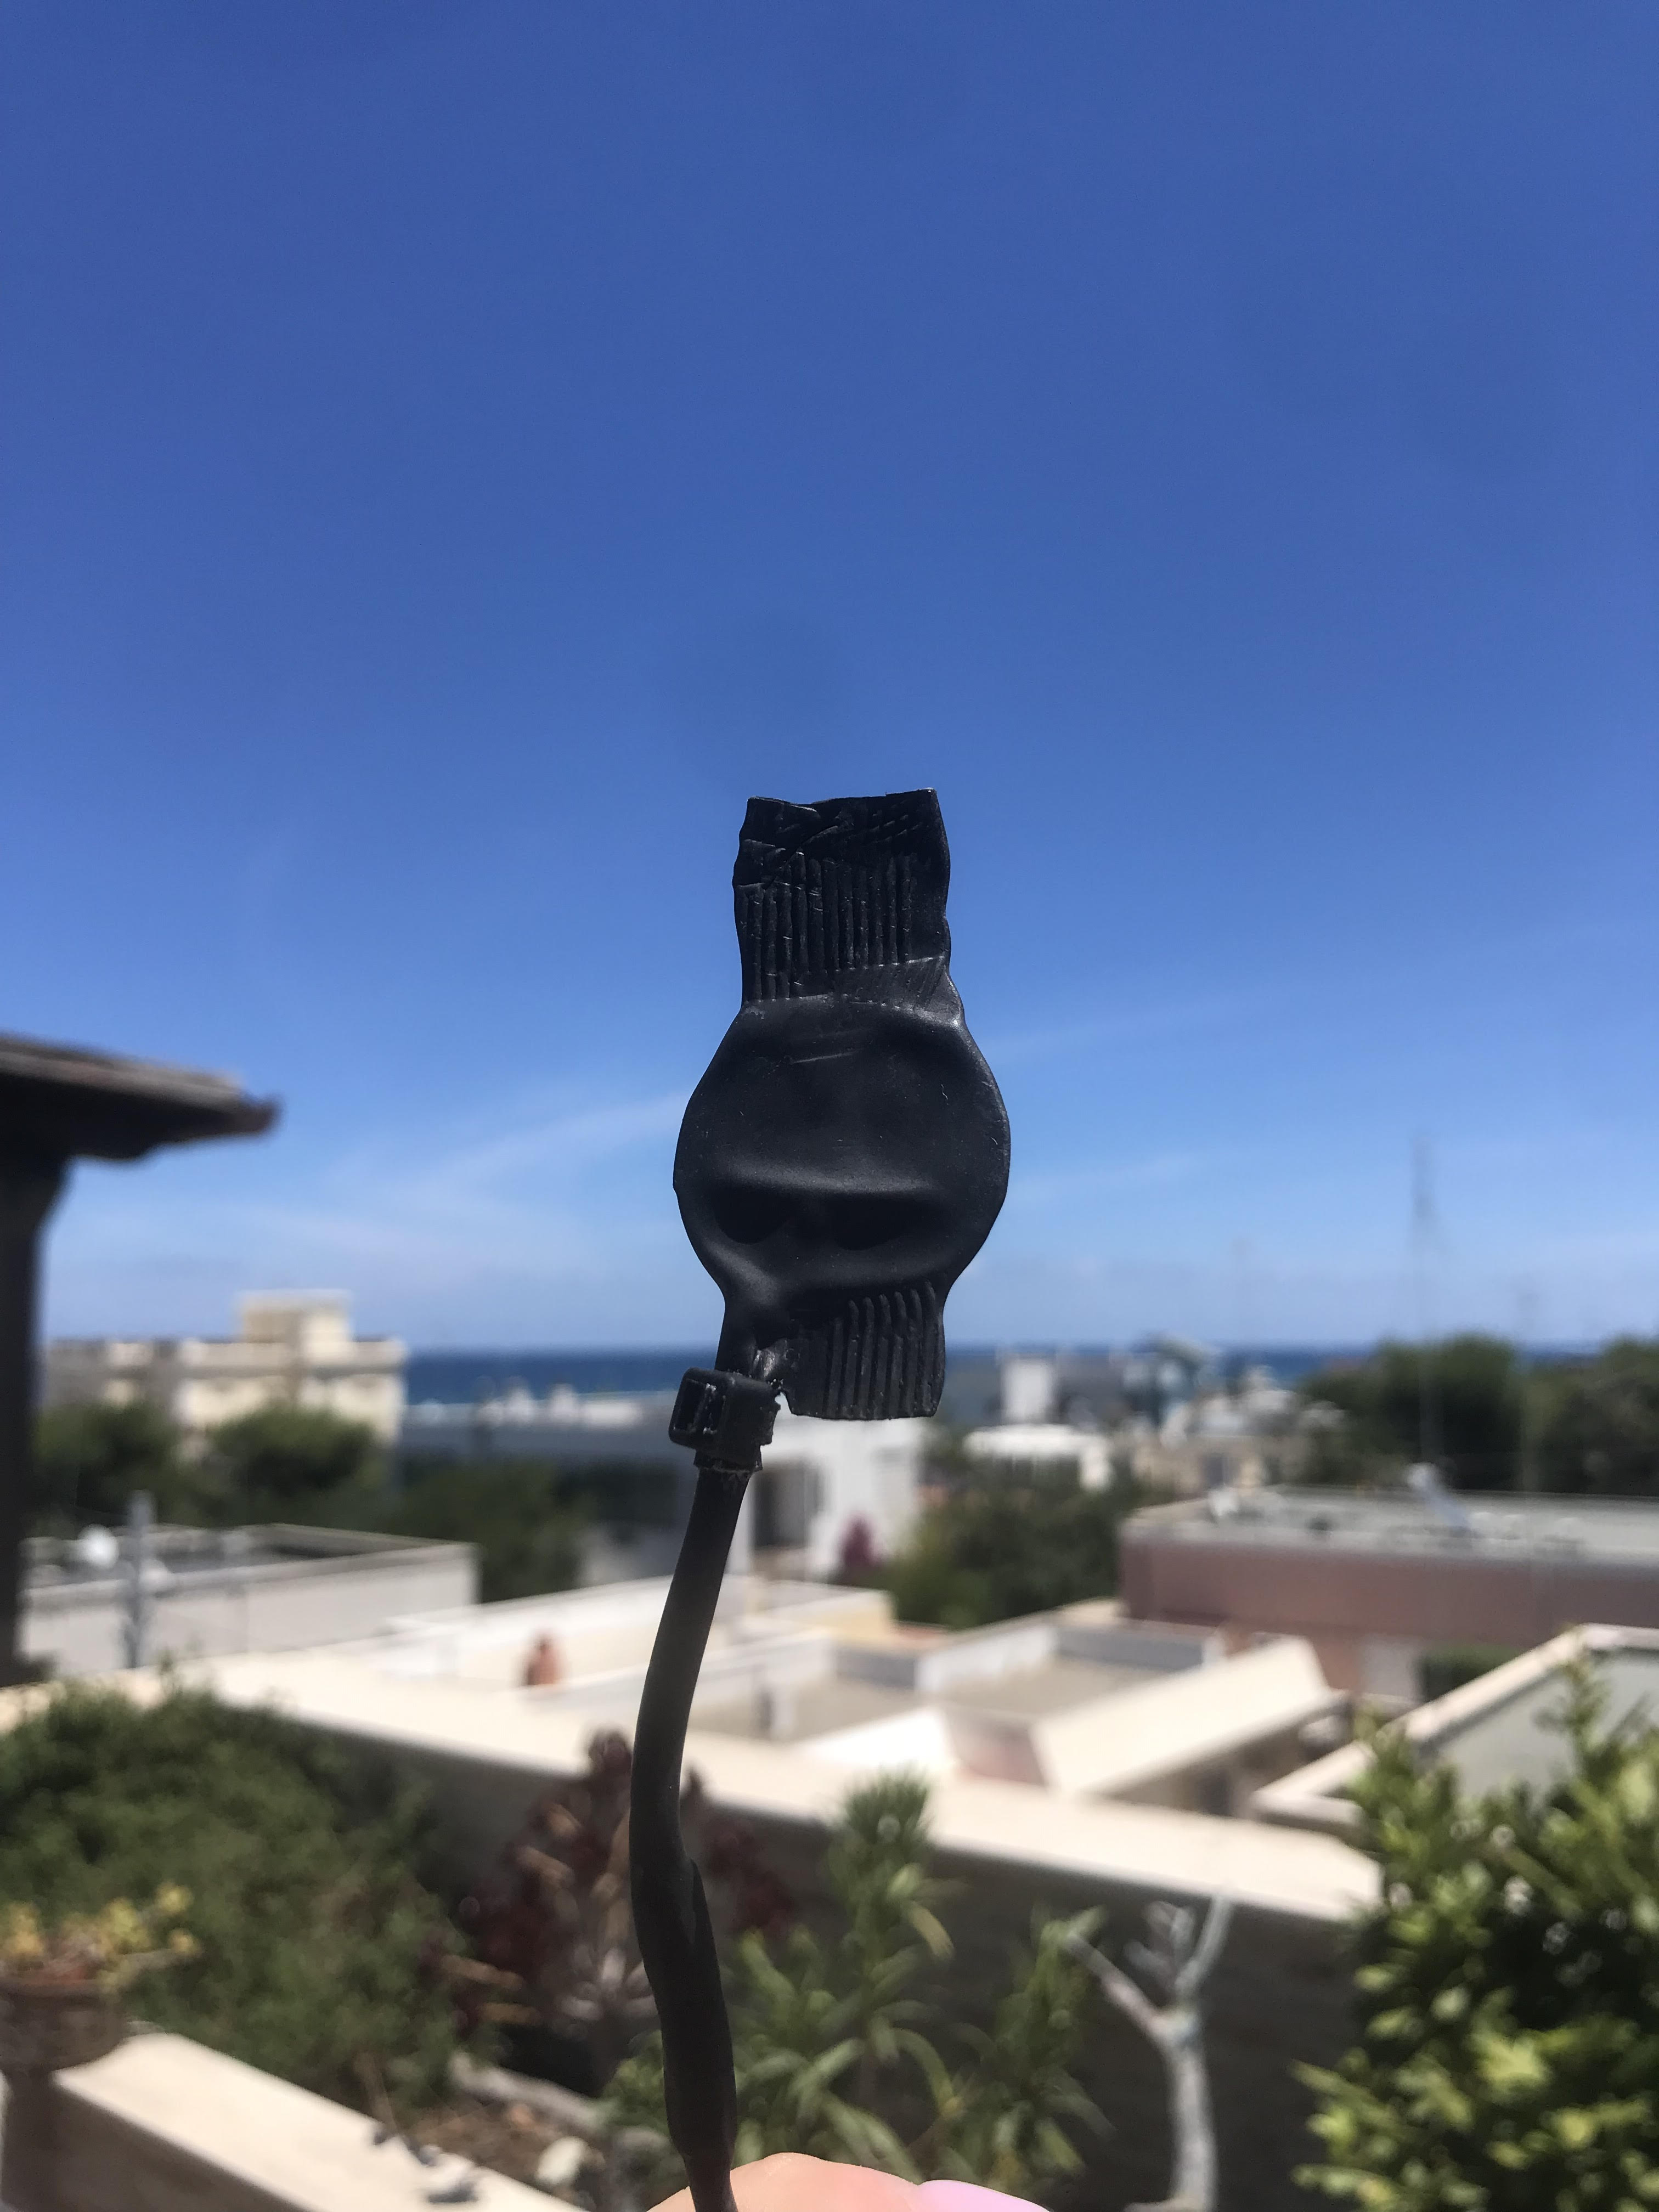
\includegraphics[width=.45\textwidth]{foto idro}} \quad

I due piezoelettrici sono stati bilanciati , positivamente e negativamente, per poi essere collegati all'interno del cavo XLR, e isolati con della plastica, proprio per utilizzarlo nell'immersione. L' idrofono DIY (do it yourself), è stato poi sottoposto a delle registrazioni in mare. Le registrazioni sono state eseguite in due luoghi differenti, Bari Santo Spirito e Molfetta. Ecco di seguito due esempi di spettrogrammi del rumore: 

\subfloat[registrazione Porto S.Spirito]
{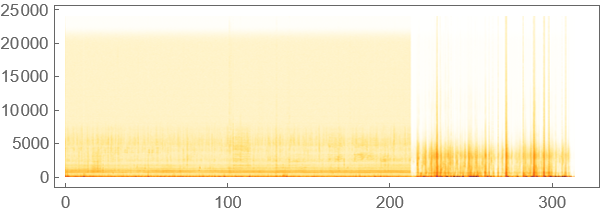
\includegraphics[width=.45\textwidth]{164431sspiritoporto}} \quad
\subfloat[registrazione Zona Militarizzata S.Spirito]
{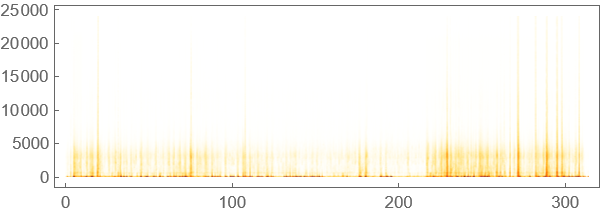
\includegraphics[width=.45\textwidth]{173608ZonaMilitarizzata}} \quad
\end{figure}

Nel primo caso, le riprese effettuate hanno riscontrato suoni e rumori, provenienti da motori di barche, rigetto di reti; La maggior parte delle registrazioni hanno ripreso rumori di fondo generali, dovuti al materiale con cui è stato costruito l'idrofono. 
Nel secondo caso, le registrazioni alla profondità di 20mt, non hanno riscontrato particolare attenzione, rumori molto bassi o quasi indefinibili. 
Proprio da questi esempi, l'utilizzo di un idrofono professionale avrebbe dato sicuramente una maggiore affidabilità a quello che è tutt'oggi l'obiettivo della ricerca. Cosa davvero provoca l'inquinamento acustico? Come il rumore contribuiscea definire inquinato il nostro mare?
Nell'immaginario collettivo, spesso l'ambiente subacqueo è totalmente privo di suoni, ma nella realtà non è così. Il mondo sottomarino è tutt'altro che silenzioso, e basta immergere la testa sott'acqua qualche secondo, per scoprirlo.
Nel linguaggio comune si parla di "rumore subacqueo", ma ciò che percepiamo, anche quando semplicemente nuotiamo in apnea, non è un singolo rumore, bensì la somma di una miriade di suoni. Sono i suoni prodotti dai numerosi organismi marini, i suoni originati dagli agenti atmosferici come il rumore delle onde e del vento, che si uniscono a loro volta ai rumori generati dalle attività umane, in certi casi particolarmente invasivi.
Per questo è più corretto parlare di "clima acustico subacqueo". 
L’ambiente marino consente al suono di percorrere notevoli distanze, nell’ordine di 1500 metri in un secondo, e ciò facilita la trasmissione, oltre che di suoni biologici, anche di tutta una vasta gamma di rumori, tra cui quelli di origine antropica, riguardo ai quali la comunità scientifica muove una sempre maggiore attenzione. Questi suoni, infatti, non interferiscono unicamente con le capacità sensoriali degli animali e la loro possibilità di comunicare, ma potrebbero anche avere una gamma più estesa di effetti, dalla morte immediata allo spostamento da abituali siti di foraggiamento ed anche di alterazione del rapporto preda/predatore o dei comportamenti riproduttivi e di orientamento. 
La Commissione Europea definisce l’inquinamento acustico sottomarino come “l’introduzione intenzionale o accidentale di energia acustica nella colonna d’acqua, da fonti puntuali o diffuse”.

Viste le scarse conoscenze specifiche sui suoi potenziali effetti si applica il "principio precauzionale" secondo cui l’assenza di certezza scientifica, qualora sussista il pericolo di danni gravi o irreversibili, non esonera gli Stati dal dovere di predisporre misure efficaci per evitare il degrado ambientale.

Per il monitoraggio del rumore subacqueo vengono presi in considerazione due indicatori:
\begin{itemize}
\item i suoni impulsivi, causati principalmente da attività esplorative a fini estrattivi e l’installazione di pali per la costruzione di piattaforme e stazioni eoliche
\item i suoni continui, generati principalmente dal trasporto marittimo
\end{itemize}

Grazie all'arpa FVG, sono riuscita ad avere contatti con MARITIME TECHNOLOGY CLUSTER FVG , Il punto di riferimento per il settore delle tecnologie marittime nel Friuli Venezia Giulia,un insieme di imprese, università, centri di ricerca, enti di formazione, il quale mi ha consigliato di contattare l'Istituto Nazionale di Oceanografia e di Geofisica Sperimentale nella provincia di Trieste. 
Grazie alla dott.ssa Tinivella, docente della sezione di Geofisica, ho avuto contatti con il CIBRA “Centro Interdisciplinare di Bioacustica”. 
Il CIBRA nasce nel 1989 come “Centro Interdisciplinare di Bioacustica” grazie al Professor Mario Pavan (1918-2003), allora Direttore dell'Istituto di Entomologia, e al Magnifico Rettore Roberto Schmid. Il Centro nasce sulle esperienze del Laboratorio di Bioacustica numerica avviato nove anni prima nell’ambito del lavoro di tesi del Dott. Gianni Pavan, e si è presto affermato come laboratorio all'avanguardia anche a livello internazionale nel settore della bioacustica e della nascente disciplina della Computational Bioacoustics. In seguito, il Centro cambia denominazione e diventa “Centro Interdisciplinare di Bioacustica e Ricerche Ambientali” per meglio indicare la valenza e le applicazioni della bioacustica nel settore ambientale, in particolare per il monitoraggio e la tutela della biodiversità.
Dalle prime ricerche strettamente di bioacustica sulle caratteristiche acustiche di singole specie, terrestri e marine, si passa a ricerche di più ampio respiro che si avvicinano ai temi dell'ecologia acustica e dell'acustica ambientale, fino a partecipare alla nascita nel 2014 di una nuova disciplina, l’Ecoacustica, che coniuga appunto bioacustica ed ecologia, e alla fondazione della International Ecoacoustic Society.
Negli ultimi anni, anche a causa dei costi elevati nel mantenere ricerche in mare, l'attenzione del CIBRA si è spostata sulla bioacustica e sull’ecoacustica come strumenti di monitoraggio ambientale terrestre e marino con la rivalutazione del concetto di Paesaggio Sonoro, tema talvolta borderline rispetto al tradizionale approccio scientifico.
il dott. Claudio Fossati Docente dell'Università di Pavia, specializzato nella ricerca del rumore del fondale marino, ha contribuito e collaborato allo ricerca di questo argomento, consegnandomi dati significativi, registrazioni provenienti dal mare della Puglia, che andremo in seguito ad analizzare. 

\subsection{Esempi}


